Next we will introduce \textit{variability parity games} (VPGs). VPGs are very similar to FPGs, they do however abstract from the notion of features and instead uses configuration for a syntactically more pleasant representation that is not solely tailored for FTSs. Furthermore in VPGs deadlocks are removed and therefore only having to reason about infinite paths and no longer about finite paths. Finally we will show the relation between VPGs and FTS verification, which is almost identical to the relation between FPGs and FTS verification.

First we introduce VPGs:
\begin{definition}
\label{def_VPG}
A variability parity game (VPG) is a tuple $(V,V_0, V_1, E, \rho, \mathfrak{C}, \theta)$, where:
\begin{itemize}
	\item $V = V_0 \cup V_1$ and $V_0 \cap V_1 = \emptyset$,
	\item $V_0$ is the set of vertices owned by player $0$,
	\item $V_1$ is the set of vertices owned by player $1$, 
	\item $E \subseteq V \times V$ is the edge relation; we assume that $E$ is total, i.e. for all $v\in V$ there is some $w \in V$ such that $(v,w) \in E$,
	\item $\rho :  V \rightarrow \mathbb{N}$ is a priority assignment,
	\item $\mathfrak{C}$ is a finite set of configurations,
	\item $\theta : E \rightarrow \mathcal{P}(\mathfrak{C})\ \backslash\ \{0\}$ is the configuration mapping, satisfying for all $v \in V$, $\bigcup\{\theta(v,w)|(v,w) \in E\} = \mathfrak{C}$.
\end{itemize}
\end{definition}
A VPG is played similarly to a PG, however the game is played for a specific configuration $c \in \mathfrak{C}$. Player $\alpha$ can only move the token from $v \in V_\alpha$ to $w \in V$ if $(v,w) \in E$ and $c \in \theta(v,w)$. Furthermore VPGs don't have deadlocks, therefore every play results in an infinite path.

A game played for configuration $c \in \mathfrak{C}$ results in winning sets $W_0^c$ and $W_1^c$, which are defined similar to the $W_0$ and $W_1$ winning sets for parity games.

\begin{definition}
\label{def_VPG_proj} The projection from VPG $G = (V, V_0, V_1, E, \rho, \mathfrak{C}, \theta)$ to a configuration $c \in \mathfrak{C}$, noted $G_{|c}$, is the parity game $(V, V_0, V_1, E', \rho)$ where $E' = \{ e\in E | c \in \theta(e)\}$.
\end{definition}

Playing VPG $G$ for a specific configuration $c \in \mathfrak{C}$ is the same as playing the PG $G_{|c}$. Any path that is valid in $G$ for $c$ is also valid in $G_{|c}$ and vice versa. Therefore the strategies are also interchangeable, furthermore the winning sets $W_\alpha$ for $G_{|c}$ and $W_\alpha^c$ for $G$ are identical. Since parity games are positionally determined so are VPGs. Similarly, since finite parity games are decidable, so are finite VPGs.
\subsection{Creating variability parity games}
We will define a translation from an FPG to a VPG. This relation is shown in the following diagram:
\\\begin{tikzpicture}
\matrix (m) [matrix of math nodes,row sep=4em,column sep=4em,minimum width=2em]
{
	\text{FPG} & \text{VPG} \\
};
\path[-stealth]
(m-1-1)
edge (m-1-2);
\end{tikzpicture}\\
To do so we have to translate products to configuration, which is trivial, furthermore we have to make the FPG deadlock free. This is done by creating two losing vertices $l_0$ and $l_1$ such that player $\alpha$ loses when the token is in vertex $l_\alpha$. Any vertex that can not move for a configuration will get an edge that is admissible for that configuration towards one of the losing vertices.
\begin{definition}
	\label{def_FPG2VPG}
	FPG2VPG($G^F$) converts FPG $G^F = (V^F, V_0^F, V_1^F, E^F, \rho^F, N, P, \gamma)$ to VPG $G = (V, V_0, V_1, E, \rho, \mathfrak{C}, \theta)$.
	
	Let $P$ be defined as  $\{p_0, p_1, \dots, p_m\}$, we define $\mathfrak{C} = \{c_0, c_1, \dots, c_m\}$.
	
	We create vertices $l_0$ and $l_1$ and define $V_0 = V_0^F \cup \{l_0\}$, $V_1 = V_1^F \cup \{l_1\}$ and $V = V_0 \cup V_1$.
	
	We construct $E$ by first making $E = E^F$ and adding edges $(l_0, l_0)$ and $(l_1, l_1)$ to $E$. Simultaneously we construct $\theta$ by first making $\theta(e) = \{c_i \in \mathfrak{C} | p_i \models \gamma(e)\}$ for every $e \in E^F$. Furthermore $\theta(l_0,l_0) = \theta(l_1,l_1) = \mathfrak{C}$.
	
	Next, for every vertex $v \in V_\alpha$ with $\alpha = \{0,1\}$, we have $C = \mathfrak{C} \backslash \bigcup \{\theta(v,w)|(v,w) \in E\}$. If $C \neq \emptyset$ then we add $(v, l_\alpha)$ to $E$ and make $\theta(v,l_\alpha) = C$.
	Finally we have 
	\[ \rho(v) = \begin{cases}
	1  & \text{if } v = l_0 \\
	0 & \text{if } v = l_1 \\
	\rho^F(v) &\text{otherwise}
	\end{cases} \]
\end{definition}
Again considering our previous working example we can translate the FPG shown in figure \ref{fig:exverfpg} to the VPG shown in figure \ref{fig:exvevpg}. Where $c_0$ corresponds to product $\emptyset$, $c_1$ corresponds to $\{f\}$ and $c_2$ to $\{f,g\}$.
\begin{figure}[h]
	\centering
	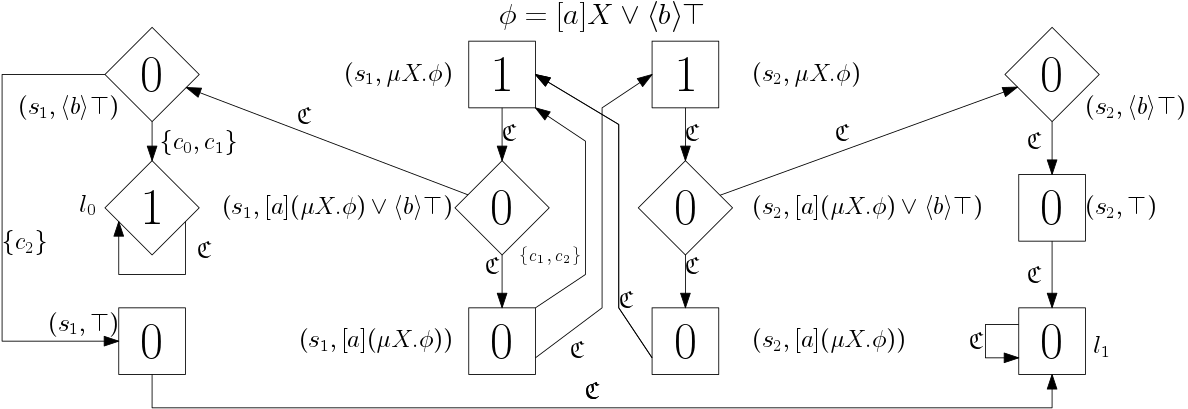
\includegraphics[scale=0.3]{Examples/ExamleVerification/VPG}
	\caption[VPG]{VPG}
	\label{fig:exvevpg}
\end{figure}

\subsection{FTS verification using VPG}
We have shown in theorem \ref{the_FPG_ver_FTS} that we can use an FPG to verify an FTS. Next we will show that a winning set in the FPG $M$ is the subset of the winning set in the VPG $FPG2VPG(M)$.
\begin{theorem}
	\label{the_FPG_sub_VPG}
	Given:
	\begin{itemize}
		\item FPG $G^F = (V^F, V_0^F, V_1^F, E^F, \rho^F, N, \{p_0, p_1, \dots, p_m\}, \gamma)$,
		\item product $p_i$
	\end{itemize}
	we have for winning sets $W_\alpha^{p_i}$ in $G$ and $W_\alpha^{c_i}$ in FPG2VPG($G^F$) that $W_\alpha^{p_i} \subseteq W_\alpha^{c_i}$ for any $\alpha \in \{0,1\}$.
	\begin{proof}
		Let $G = (V,V_0,V_1, E, \rho, \mathfrak{C},\theta) =$ FPG2VPG($G^F$). Consider finite play $\pi$ that is valid in game $G^F$ for product $p_i$. We have for every $(\pi_i, \pi_{i+1})$ in $\pi$ that $(\pi_i, \pi_{i+1}) \in E^F$ and $p_i \models \gamma((\pi_i, \pi_{i+1}))$. From the $FPG2VPG$ definition (\ref{def_FPG2VPG}) it follows that $(\pi_i, \pi_{i+1}) \in E$ and $c_i \in \theta(\pi_i, \pi_{i+1})$. So we can conclude that path $\pi$ is also valid in game $G$ for configuration $c_i$. Since the play is finite the winner is determined by the last vertex $v$ in $\pi$, player $\alpha$ wins such that $v \in V_{\overline{\alpha}}$. Furthermore we know, because the play is finite, that there exists no $(v,w) \in E^F$ with $p \models \gamma(v,w)$. From this we can conclude that $(v, l_{\overline{\alpha}}) \in E$ and $c_i \in \theta(v, l_{\overline{\alpha}})$. Vertex $l_{\overline{\alpha}}$ has one outgoing edge, namely to itself. So finite play $\pi$ will in game $G^F$ results in an infinite play $\pi(l_{\overline{\alpha}})^\omega$. Vertex $l_{\overline{\alpha}}$ has a priority with the same parity as player $\alpha$, so player $\alpha$ wins the infinite play in $G$ for configuration $c_i$.
		
		Consider infinite play $\pi$ that is valid in game $G^F$ for product $p_i$. As shown above this play is also valid in game $G$ for configuration $c_i$. Since the win conditions of both games are the same the play will result in the same winner.
		
		Consider infinite play $\pi$ that is valid in game $G$ for configuration $c_i$. We distinguish two cases:
		\begin{itemize}
			\item If $l_\alpha$ doesn't occur in $\pi$ then the path is also valid for game $G^F$ with product $p_i$ and has the same winner.
			\item If $\pi = \pi'(l_\alpha)^\omega$ with no occurrence $l_\alpha$ in $\pi'$ then the winner is player $\overline{\alpha}$. The path $\pi'$ is valid for game $G^F$ with product $p_i$. Let vertex $v$ be the last vertex of $\pi'$. Since $(v, l_\alpha) \in E$ and $c_i \in \theta(v,l_\alpha)$ we know that there is no $(v,w) \in E^F$ with $p_i \models \gamma(v,w)$ and that vertex $v$ is owned by player $\alpha$. So in game $G^F$ player $\alpha$ can't move at vertex $v$ and therefore loses the game (in which case the winner is also $\overline{\alpha}$.
		\end{itemize}
		
		We have shown that every path (finite or infinite) in game $G^F$ with product $p_i$ can be played in game $G$ with configuration $c_i$ and that they have the same winner. Furthermore every infinite path in game $G$ with configuration $c_i$ can be either played as an infinite path or the first part of the path can be played in $G^F$ with product $p_i$ and they have the same winner. From this we can conclude that the theorem holds.
	\end{proof}
\end{theorem}
We can conclude the diagram depicting the relation between the different games and transition systems:\\
\begin{tikzpicture}
\matrix (m) [matrix of math nodes,row sep=4em,column sep=4em,minimum width=2em]
{
	\text{FTS} & \text{FPG} & \text{VPG} \\
	\text{LTS} & \text{PG} \\};
\path[-stealth]
(m-1-1) edge [double] node [left] {$\Pi$} (m-2-1)
edge node [above] {$\varphi$} (m-1-2)
(m-2-1.east|-m-2-2) edge node [above] {$\varphi$}
(m-2-2)
(m-1-2) edge [double] node [right] {$\Pi$} (m-2-2)
edge (m-1-3);
\end{tikzpicture}\\
Finally we show that VPGs can be used to verify FPGs.
\begin{theorem}
	\label{the_VPG_ver_FTS}
	Given:
	\begin{itemize}
		\item FTS $M = (S, Act, trans, s_0, N, \{p_0,\dots,p_m\}, \gamma)$,
		\item closed modal mu-calculus formula $\varphi$,
		\item product $p_i \in P$ and
		\item state $s \in S$
	\end{itemize}
	it holds that $M_{|p_i}, s \models \varphi$ if and only if $(s, \varphi) \in W_0^{c_i}$ in $FPG2VPG(FTS2FPG(M, \varphi))$.
	\begin{proof}
		Using theorem \ref{the_FPG_ver_FTS} we find that $M_{|p_i}, s \models \varphi$ if and only if $(s, \varphi) \in W_0^{p_i}$ for game $FTS2FPG(M, \varphi)$. If $(s, \varphi) \in W_0^{p_i}$ then we find by using theorem \ref{the_FPG_sub_VPG} that $(s, \varphi) \in W_0^{c_i}$ for game $FPG2VPG(FTS2FPG(M, \varphi))$. If $(s, \varphi) \not\in W_0^{p_i}$ then $(s, \varphi) \in W_1^{p_i}$ and therefore $(s, \varphi) \in W_1^{c_i}$ for game $FPG2VPG(FTS2FPG(M, \varphi))$ and $(s, \varphi) \not\in W_0^{c_i}$.
	\end{proof}
\end{theorem}
This theorem concludes the model verification technique depicted in figure \ref{fig:ftsverificationusingvpg}.